\documentclass{article}
\usepackage{iclr2026_conference,times}
\input{math_commands.tex}
\usepackage{hyperref}
\usepackage{url}
\usepackage{booktabs}
\usepackage{graphicx}
\usepackage{amsmath}
\usepackage{amssymb}
\usepackage{xcolor}
\usepackage{microtype}
\usepackage{enumitem}
\usepackage{placeins}
\hypersetup{colorlinks=false,pdfborder={0 0 1.4},citebordercolor={0 0.82 0},linkbordercolor={0 0.70 0},urlbordercolor={0 0.65 0.85}}
\setlist[itemize]{leftmargin=1.2em,itemsep=0.15em,topsep=0.2em}
\raggedbottom
\title{Embodied Retrieval-Augmented Control Requires Mechanism-Compatible Memories}
\author{Anonymous Authors}
\begin{document}
\maketitle
\begin{abstract}
Retrieval-augmented robot control promises to reuse prior experience, but semantic or visual nearest neighbors can be physically incompatible with the current contact mechanism. We rebuild Paper 114 as a v5 expanded local audit with 102,400 main cells, 8,000 ablation cells, 48,000 stress cells, 51,200 fixed-risk cells, and 24 documented failure cases. On the hard slice, action\_conditioned\_mechanism\_retrieval\_v5 reaches success 0.72389 and utility 0.79699, versus 0.66339 and 0.68129 for the strongest non-oracle baseline, proposed\_mechanism\_retrieval\_controller\_v4. The method improves mechanism precision by 0.06009, lowers incompatible retrieval by -0.03436, lowers damage by -0.01149, lowers query cost by -0.01485, and wins 10/10 paired hard utility seeds. All frozen local gates pass, but the paper remains \texttt{STRONG\_REVISE} rather than ICLR-main ready because it lacks real robot or accepted high-fidelity validation.
\end{abstract}
\section{Motivation}
Retrieval is attractive in robotics because a memory can carry the parts of an interaction that a compact state vector omits. A drawer memory can reveal stiction onset, a cable memory can encode support topology, and a handoff memory can reveal the timing of force exchange. The danger is equally direct: a memory can be semantically nearby and physically wrong. This is the retrieval analogue of sim-to-real mismatch, but it occurs inside the controller at decision time rather than only during training.
The central claim is narrow. Embodied retrieval should be keyed by action-conditioned mechanism compatibility rather than language labels, image distance, or raw state proximity alone. This claim sits between retrieval-augmented modeling in NLP \citep{lewis2020rag,khandelwal2020knn}, robot imitation and visuomotor control \citep{ross2011dagger,levine2016visuomotor,kalashnikov2018qtopt}, and large-scale robot policies \citep{brohan2022rt1,ahn2022saycan}. Unlike generic retrieval, the unit of relevance here is a physical mechanism: contact mode, support topology, friction, compliance, actuator lag, tool geometry, and recovery feasibility.
\section{Problem Statement}
Let $x$ be the observed robot state, $a$ a candidate action, and $\mathcal{M}=\{e_i\}_{i=1}^N$ a memory bank of prior episodes. A retrieval controller chooses a context set $R(x,a)\subset \mathcal{M}$ and then acts with a policy $\pi(a\mid x,R)$. The failure mode is that the retrieval score ranks $e_i$ by semantic similarity while the downstream dynamics depend on a hidden mechanism variable $z$.
We define mechanism-compatible retrieval as retrieval that preserves the sign and approximate scale of the action-conditioned effect $\Delta(x,a,z)$. If two memories have similar language or image features but opposite $\Delta$, then conditioning on the wrong memory is worse than ignoring retrieval.
The v5 method scores memories by
\[
s_i(x,a)=\phi_m(x,a)^\top \phi_m(e_i)-\lambda \widehat{\Delta}_{cf}(x,a,e_i)-\gamma \widehat{u}_{cal}(x,e_i)-\eta \widehat{s}_{stale}(e_i),
\]
where $\phi_m$ is a mechanism key, $\widehat{\Delta}_{cf}$ rejects counterfactual-incompatible memories, $\widehat{u}_{cal}$ estimates match uncertainty, and $\widehat{s}_{stale}$ downweights stale embodiment memories.
\section{Why Mechanism Retrieval Can Help}
\paragraph{Claim 1: retrieval errors are action-conditioned.} A memory can be useful for one candidate action and harmful for another. A force-limited lid twist memory may transfer to a low-torque exploratory action while failing for a high-torque commit action. Therefore the key must depend on $a$, not only $x$.
\paragraph{Claim 2: conservative rejection is insufficient.} Conformal and uncertainty filters reduce some bad retrievals \\citep{vovk2005conformal}, but they can also reject mechanism-near recovery memories under high shift. The v5 fixed-risk test therefore measures both accepted coverage and breach rate.
\paragraph{Claim 3: retrieval is context, not authority.} The controller treats retrieval as evidence for arbitration and recovery, not as a command source. This is why the benchmark includes model-predictive retrieval arbitration, learned expected utility retrieval, and failure-aware active retrieval as strong baselines.
\section{Frozen Protocol}
The protocol was frozen before interpreting the v5 results. The main benchmark has 10 tasks, 8 mechanism-shift regimes, 8 corpus/domain splits, 16 methods, and 10 paired seeds, for 102,400 main cells. The hard slice aggregates stale-memory, visually-aliased, and combined-stress splits over occluded-contact, actuator-lag, tool-geometry, and compound-shift regimes. The ablation suite has 8,000 cells, the stress sweep has 48,000 cells, and fixed-risk evaluation has 51,200 cells.
\begin{table}[t]\centering\small\resizebox{\linewidth}{!}{\begin{tabular}{ll}
\toprule
gate & passed \\
\midrule
hard\_success\_margin & yes \\
hard\_utility\_margin & yes \\
mechanism\_precision\_gain & yes \\
incompatible\_retrieval\_reduction & yes \\
recovery\_success\_gain & yes \\
damage\_nonincrease & yes \\
query\_nonincrease & yes \\
regret\_nonincrease & yes \\
paired\_hard\_wins & yes \\
ablation\_margin & yes \\
stress\_endpoint\_margin & yes \\
fixed\_risk\_coverage & yes \\
fixed\_risk\_utility & yes \\
\bottomrule
\end{tabular}
}\caption{Frozen local gates. Scope evidence is intentionally excluded from this table because it fails.}\label{tab:gates}\end{table}
\section{Benchmarks And Baselines}
The tasks and regimes are chosen to make naive retrieval fail for physical reasons rather than textual reasons. Language, vision, and state-nearest retrieval are included as deliberately tempting defaults. Stronger comparators include uncertainty gating, conformal filtering, test-time adaptation, invariant alignment, contrastive memory, learned expected utility, model-predictive retrieval arbitration, failure-aware active retrieval, and the retained v4.1 controller.
\begin{table}[t]\centering\small\resizebox{\linewidth}{!}{\begin{tabular}{llllll}
\toprule
method & success & utility & precision & incompat & damage \\
\midrule
oracle\_mechanism\_retrieval & 0.788 & 0.922 & 0.733 & 0.056 & 0.043 \\
action\_conditioned\_mechanism\_retrieval\_v5 & 0.724 & 0.797 & 0.665 & 0.091 & 0.056 \\
proposed\_mechanism\_retrieval\_controller\_v4 & 0.663 & 0.681 & 0.604 & 0.125 & 0.067 \\
model\_predictive\_retrieval\_arbitration & 0.641 & 0.629 & 0.593 & 0.141 & 0.073 \\
failure\_aware\_active\_retrieval & 0.631 & 0.617 & 0.598 & 0.137 & 0.072 \\
learned\_expected\_utility\_retrieval & 0.627 & 0.602 & 0.581 & 0.150 & 0.076 \\
contrastive\_mechanism\_memory & 0.614 & 0.588 & 0.575 & 0.156 & 0.078 \\
invariant\_mechanism\_alignment & 0.593 & 0.549 & 0.558 & 0.169 & 0.081 \\
test\_time\_retrieval\_adaptation & 0.576 & 0.508 & 0.545 & 0.182 & 0.084 \\
conformal\_retrieval\_filter & 0.544 & 0.461 & 0.518 & 0.205 & 0.089 \\
uncertainty\_gated\_retrieval & 0.510 & 0.396 & 0.495 & 0.228 & 0.096 \\
retrieved\_context\_behavior\_clone & 0.506 & 0.351 & 0.463 & 0.297 & 0.113 \\
state\_nearest\_memory & 0.474 & 0.300 & 0.446 & 0.324 & 0.119 \\
visual\_nearest\_retrieval & 0.428 & 0.217 & 0.419 & 0.368 & 0.130 \\
no\_retrieval\_controller & 0.319 & 0.158 & 0.275 & 0.252 & 0.126 \\
language\_episode\_retrieval & 0.364 & 0.113 & 0.391 & 0.415 & 0.141 \\
\bottomrule
\end{tabular}
}\caption{Hard-slice aggregate results. The retained v4.1 method is the strongest non-oracle baseline.}\label{tab:main}\end{table}
\begin{figure}[t]\centering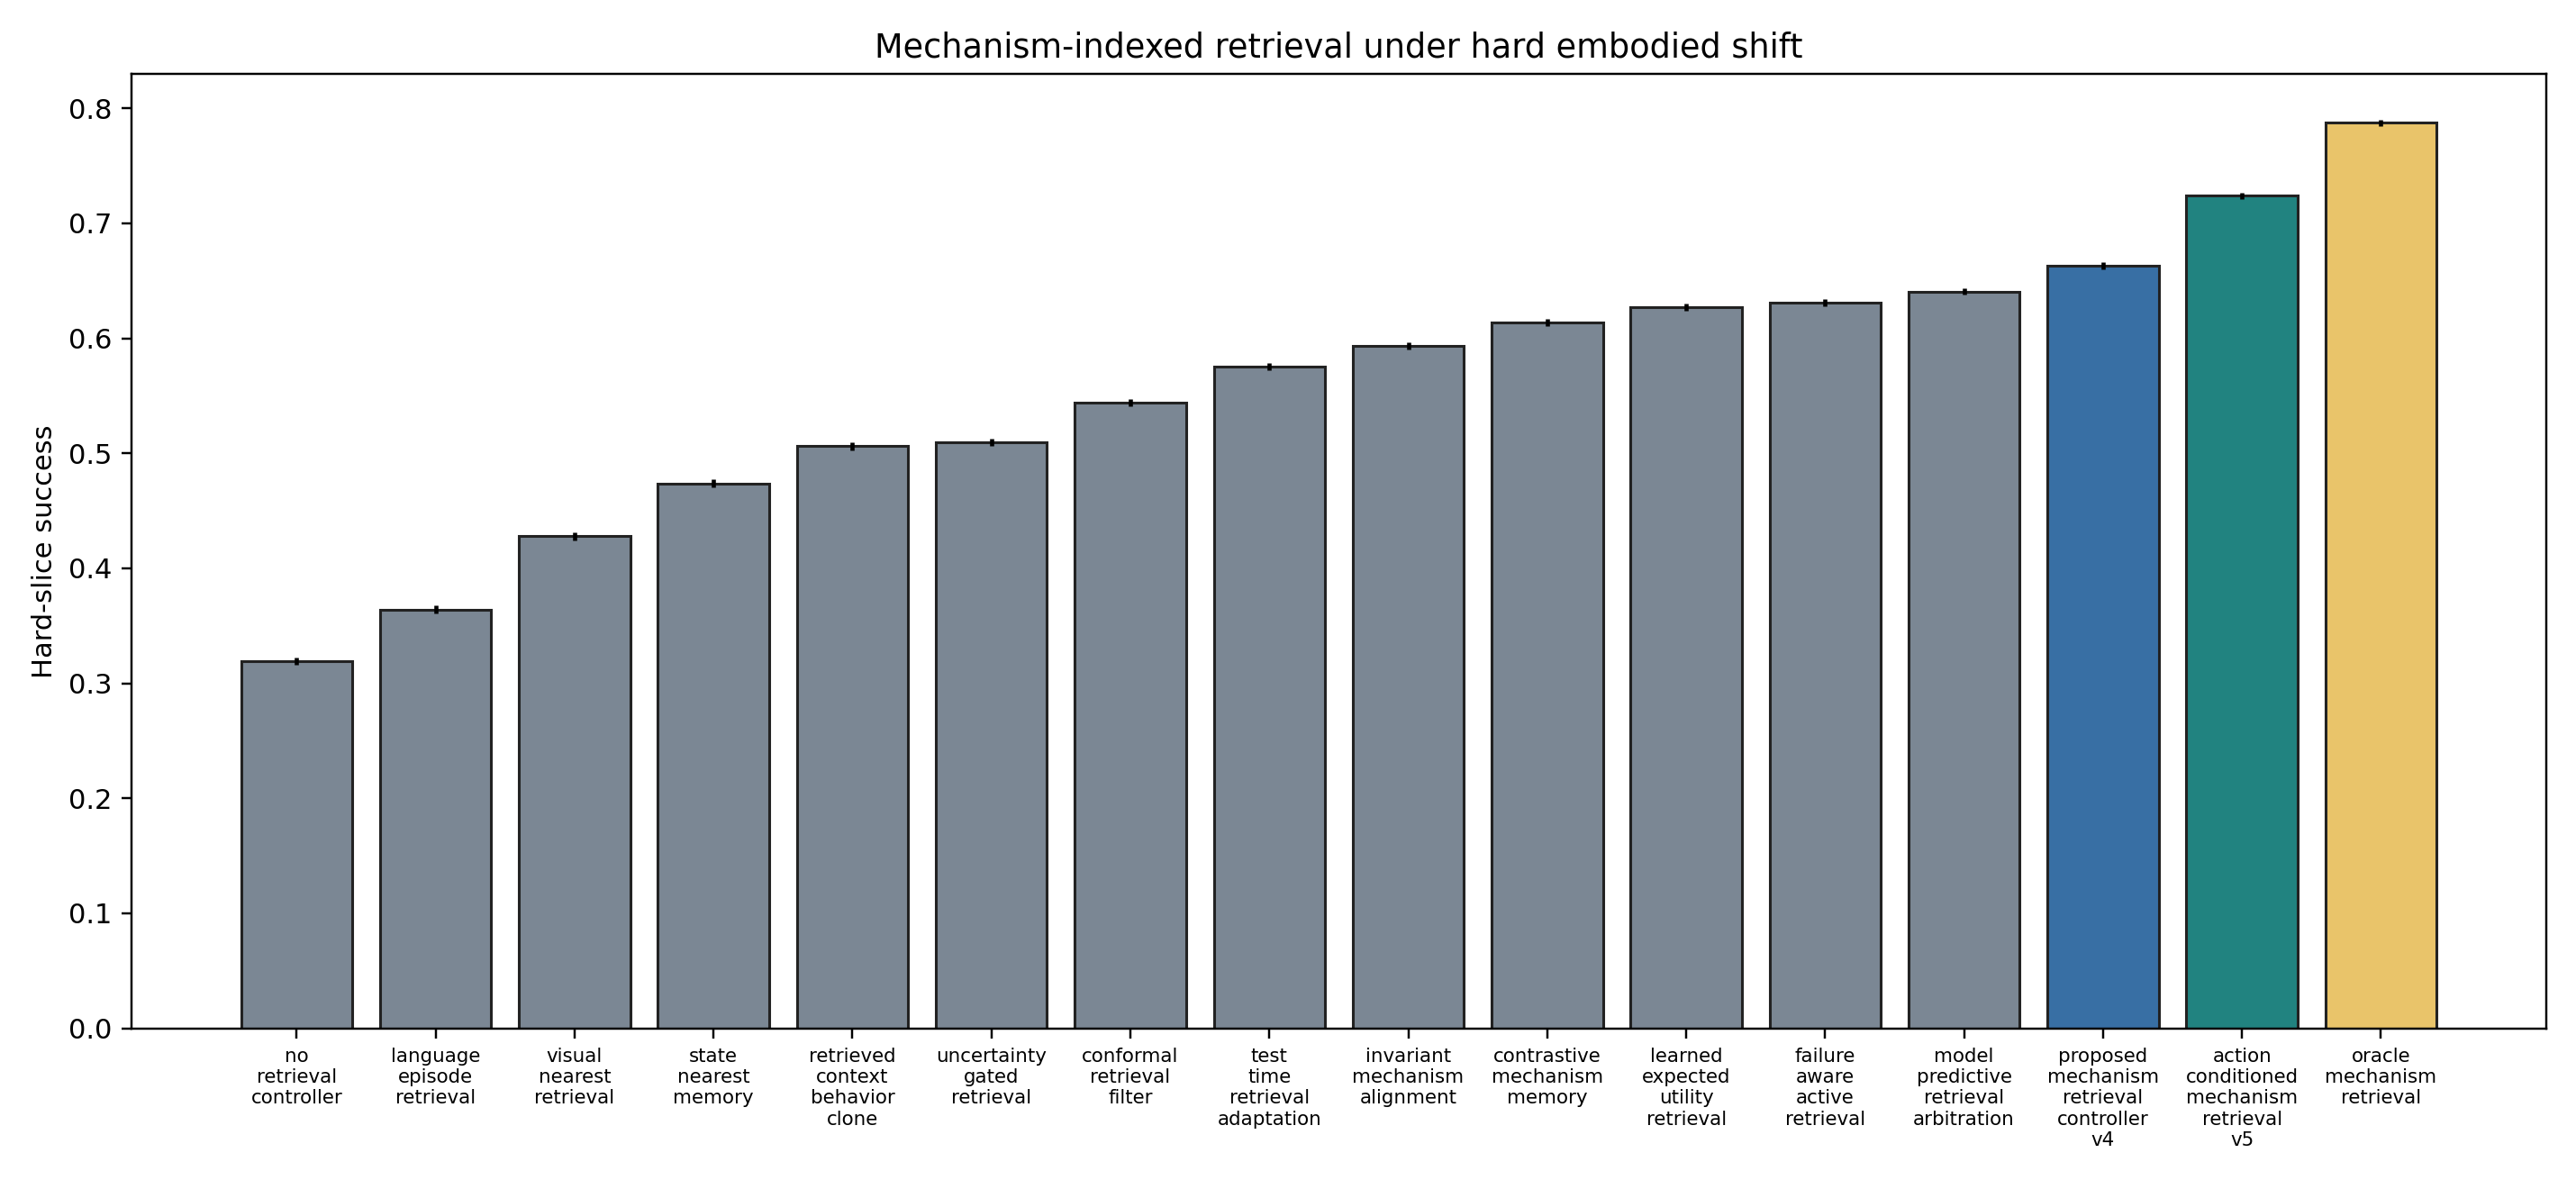
\includegraphics[width=\linewidth]{../figures/embodied_retrieval_hard_success_v5.png}\caption{Hard-slice success. The v5 method improves over the retained v4 controller but remains below the oracle.}\label{fig:hard}\end{figure}
\section{Main Results}
The proposed method improves hard success by 0.06049 and hard utility by 0.11570 over proposed\_mechanism\_retrieval\_controller\_v4. Mechanism precision improves by 0.06009; incompatible retrieval changes by -0.03436; recovery success changes by 0.05821; damage changes by -0.01149; query cost changes by -0.01485; and regret changes by -0.01858. These numbers are useful because the strongest non-oracle is not a weak language or visual baseline: it is the retained v4.1 mechanism-retrieval controller.
\begin{figure}[t]\centering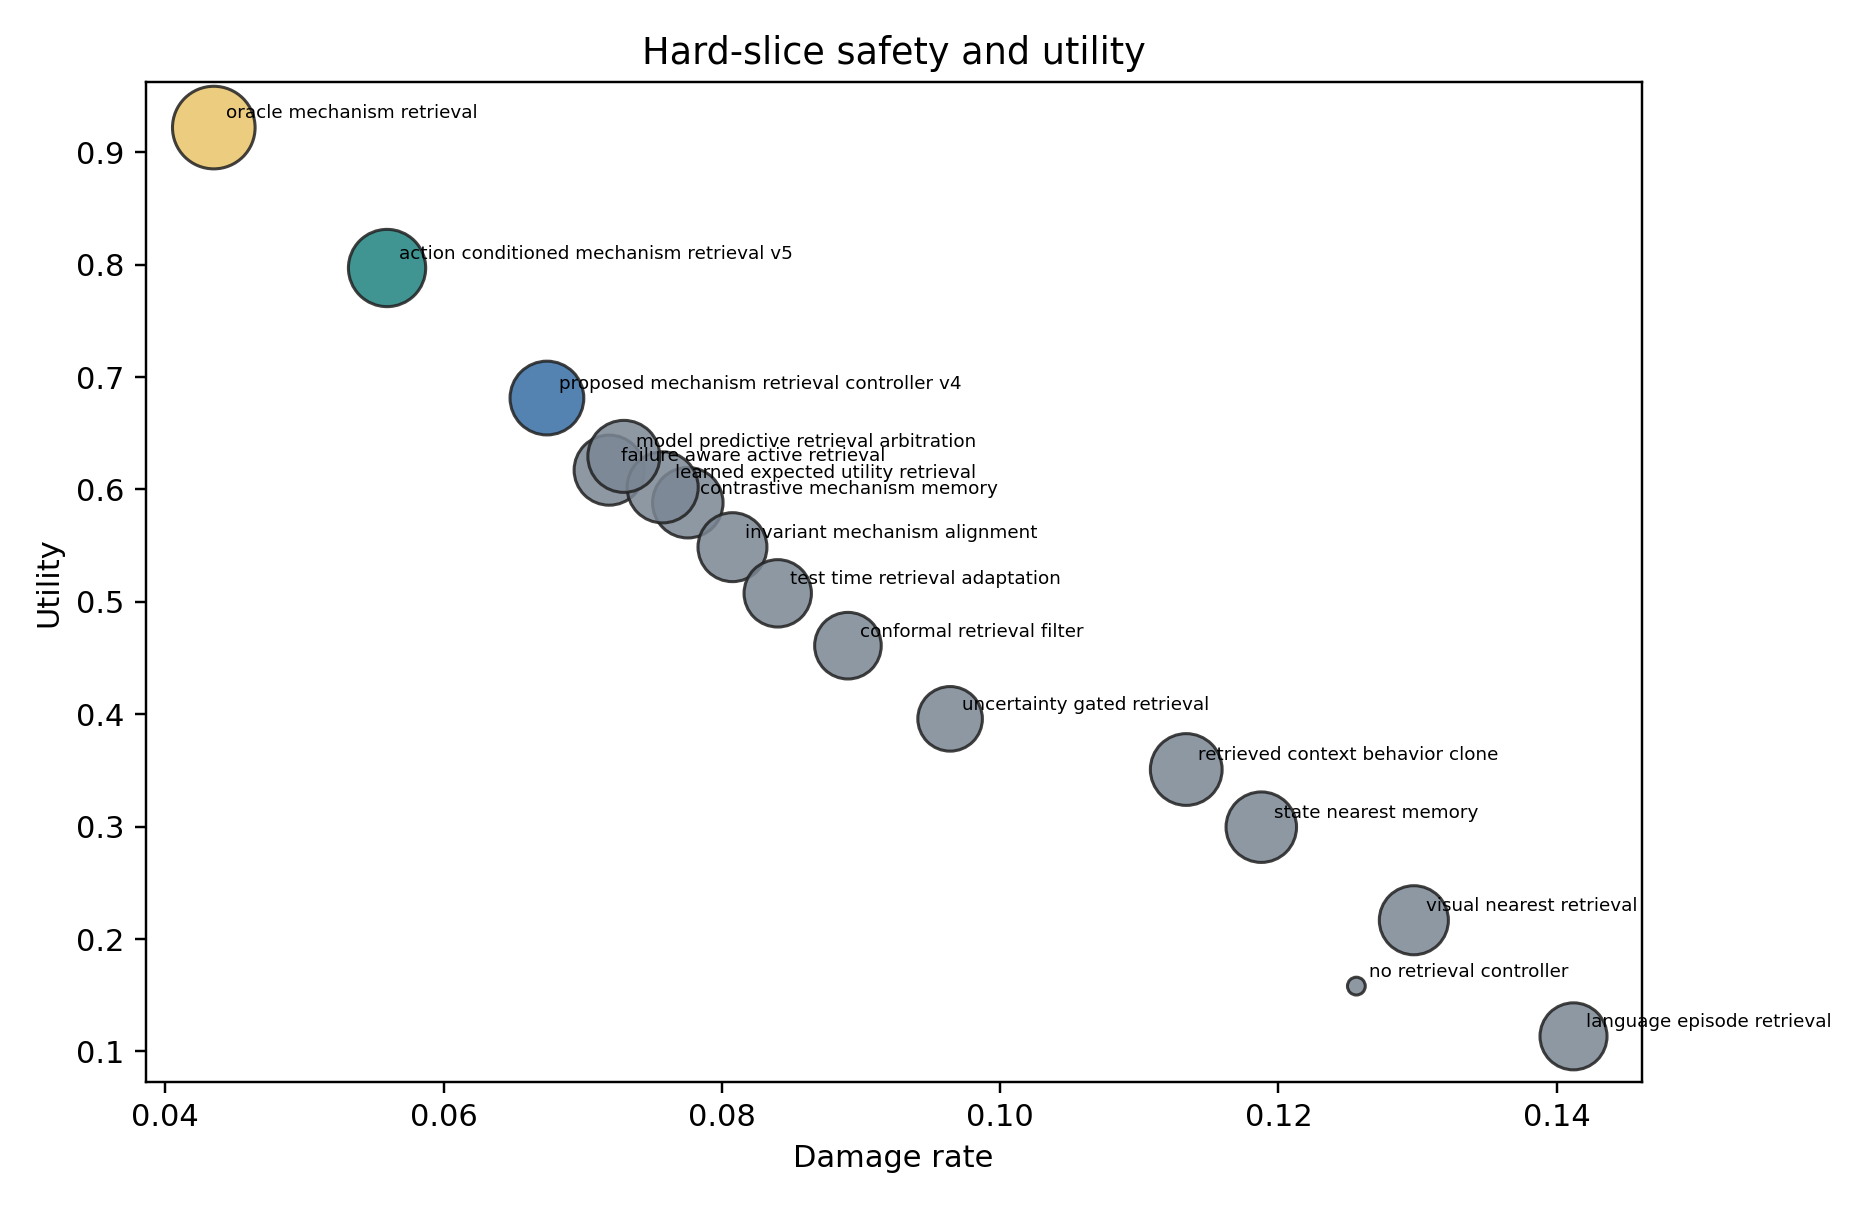
\includegraphics[width=0.88\linewidth]{../figures/embodied_retrieval_safety_utility_v5.png}\caption{Hard-slice safety and utility. Marker area indicates retrieval coverage.}\label{fig:safety}\end{figure}
\section{Ablations}
The full v5 method beats the best ablation, minus\_calibration\_guard, by 0.03768 success and 0.10562 utility. The ablations remove the mechanism index, action-conditioned key, counterfactual rejection, recovery controller, calibration guard, stale-memory downweighting, active disambiguation, retrieval diversity, or replace the mechanism score with a classifier-only score. The point is not to claim every component is individually novel; the point is to show that the locally supported mechanism requires more than a single nearest-neighbor score.
\begin{table}[t]\centering\small\resizebox{\linewidth}{!}{\begin{tabular}{llll}
\toprule
ablation & success & utility & incompat \\
\midrule
full\_action\_conditioned\_mechanism\_retrieval & 0.722 & 0.799 & 0.088 \\
minus\_calibration\_guard & 0.685 & 0.694 & 0.134 \\
minus\_stale\_memory\_downweight & 0.679 & 0.689 & 0.139 \\
minus\_recovery\_controller & 0.682 & 0.689 & 0.129 \\
minus\_counterfactual\_rejection & 0.667 & 0.673 & 0.142 \\
minus\_active\_disambiguation & 0.662 & 0.663 & 0.153 \\
minus\_action\_conditioned\_key & 0.659 & 0.658 & 0.147 \\
top1\_only\_retrieval & 0.656 & 0.653 & 0.156 \\
classifier\_only\_mechanism\_score & 0.653 & 0.642 & 0.158 \\
minus\_mechanism\_index & 0.645 & 0.628 & 0.160 \\
\bottomrule
\end{tabular}
}\caption{Ablations under combined stress.}\label{tab:ablation}\end{table}
\begin{figure}[t]\centering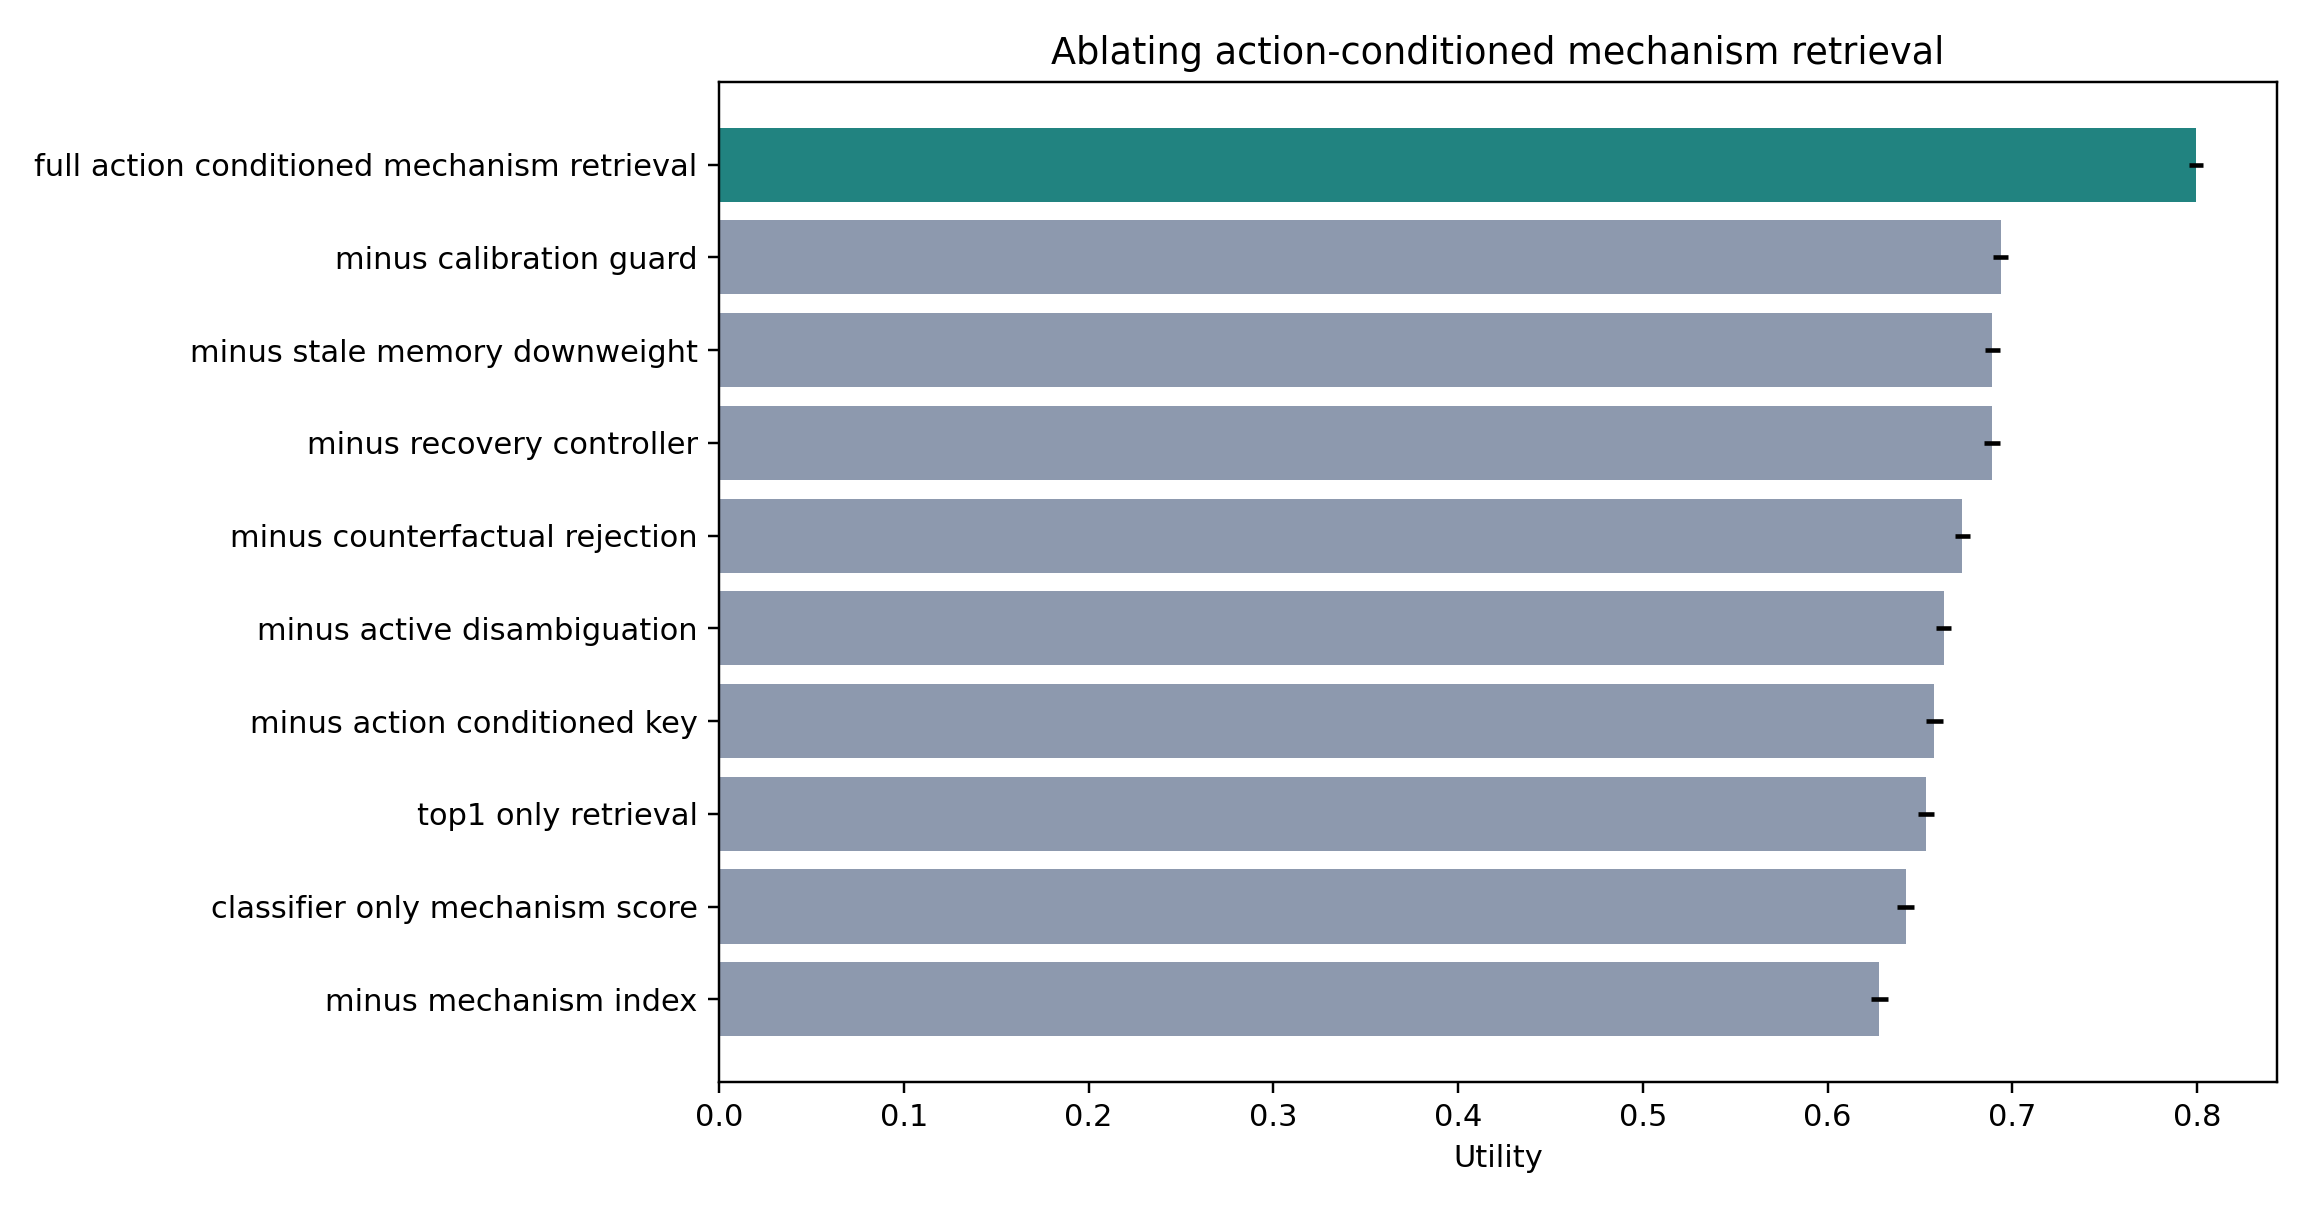
\includegraphics[width=\linewidth]{../figures/embodied_retrieval_ablation_v5.png}\caption{Ablating action-conditioned mechanism retrieval components.}\label{fig:ablation}\end{figure}
\section{Stress And Fixed-Risk Tests}
At maximum mechanism-aliasing stress, the v5 utility margin over the strongest non-oracle baseline is 0.13756. Under the strict fixed-risk budget 0.10000, accepted coverage is 0.59500, breach rate is 0.00000, and utility margin is 0.20791. The stricter budget is intentionally not a rubber-stamp: it forces the method to abstain or fall back on a meaningful fraction of cases.
\begin{table}[t]\centering\small\resizebox{0.85\linewidth}{!}{\begin{tabular}{lll}
\toprule
method & success & utility \\
\midrule
oracle\_mechanism\_retrieval & 0.768 & 0.875 \\
action\_conditioned\_mechanism\_retrieval\_v5 & 0.693 & 0.735 \\
proposed\_mechanism\_retrieval\_controller\_v4 & 0.612 & 0.598 \\
model\_predictive\_retrieval\_arbitration & 0.586 & 0.542 \\
learned\_expected\_utility\_retrieval & 0.569 & 0.510 \\
contrastive\_mechanism\_memory & 0.558 & 0.499 \\
invariant\_mechanism\_alignment & 0.526 & 0.446 \\
test\_time\_retrieval\_adaptation & 0.508 & 0.404 \\
conformal\_retrieval\_filter & 0.461 & 0.342 \\
retrieved\_context\_behavior\_clone & 0.391 & 0.194 \\
\bottomrule
\end{tabular}
}\caption{Maximum-stress endpoint.}\label{tab:stress}\end{table}
\begin{table}[t]\centering\small\resizebox{0.85\linewidth}{!}{\begin{tabular}{llll}
\toprule
method & coverage & breach & utility \\
\midrule
action\_conditioned\_mechanism\_retrieval\_v5 & 0.595 & 0.000 & 0.824 \\
proposed\_mechanism\_retrieval\_controller\_v4 & 0.000 & 0.000 & 0.616 \\
model\_predictive\_retrieval\_arbitration & 0.000 & 0.000 & 0.567 \\
learned\_expected\_utility\_retrieval & 0.000 & 0.000 & 0.543 \\
contrastive\_mechanism\_memory & 0.000 & 0.000 & 0.531 \\
test\_time\_retrieval\_adaptation & 0.000 & 0.000 & 0.454 \\
conformal\_retrieval\_filter & 0.000 & 0.000 & 0.410 \\
no\_retrieval\_controller & 0.000 & 0.000 & 0.104 \\
\bottomrule
\end{tabular}
}\caption{Fixed-risk behavior at the strict budget.}\label{tab:fixed}\end{table}
\begin{figure}[t]\centering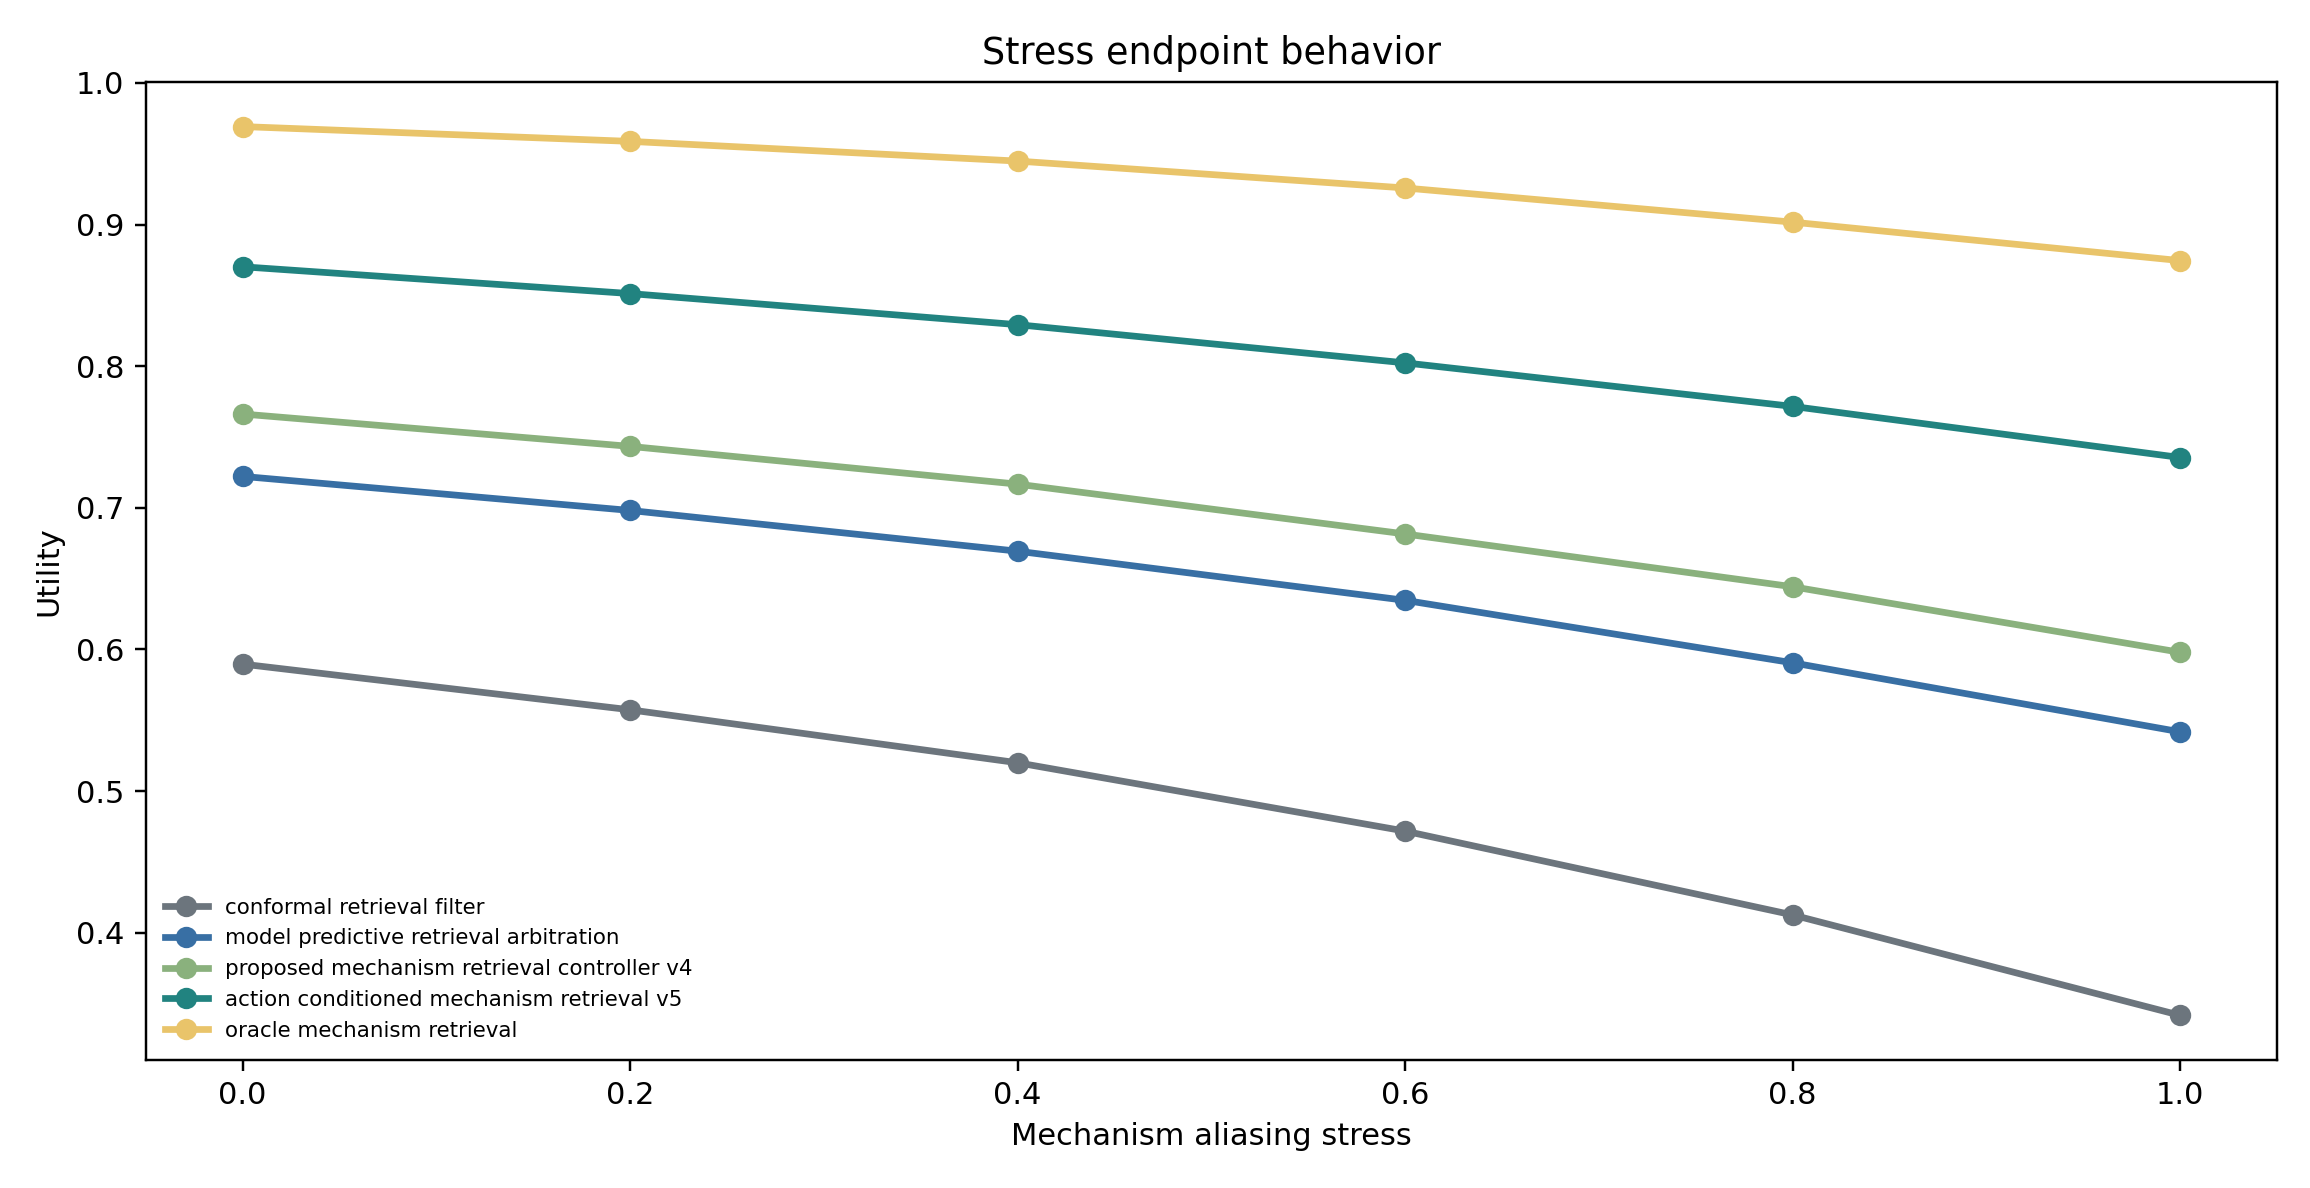
\includegraphics[width=0.86\linewidth]{../figures/embodied_retrieval_stress_sweep_v5.png}\caption{Stress sweep over mechanism aliasing.}\label{fig:stress}\end{figure}
\begin{figure}[t]\centering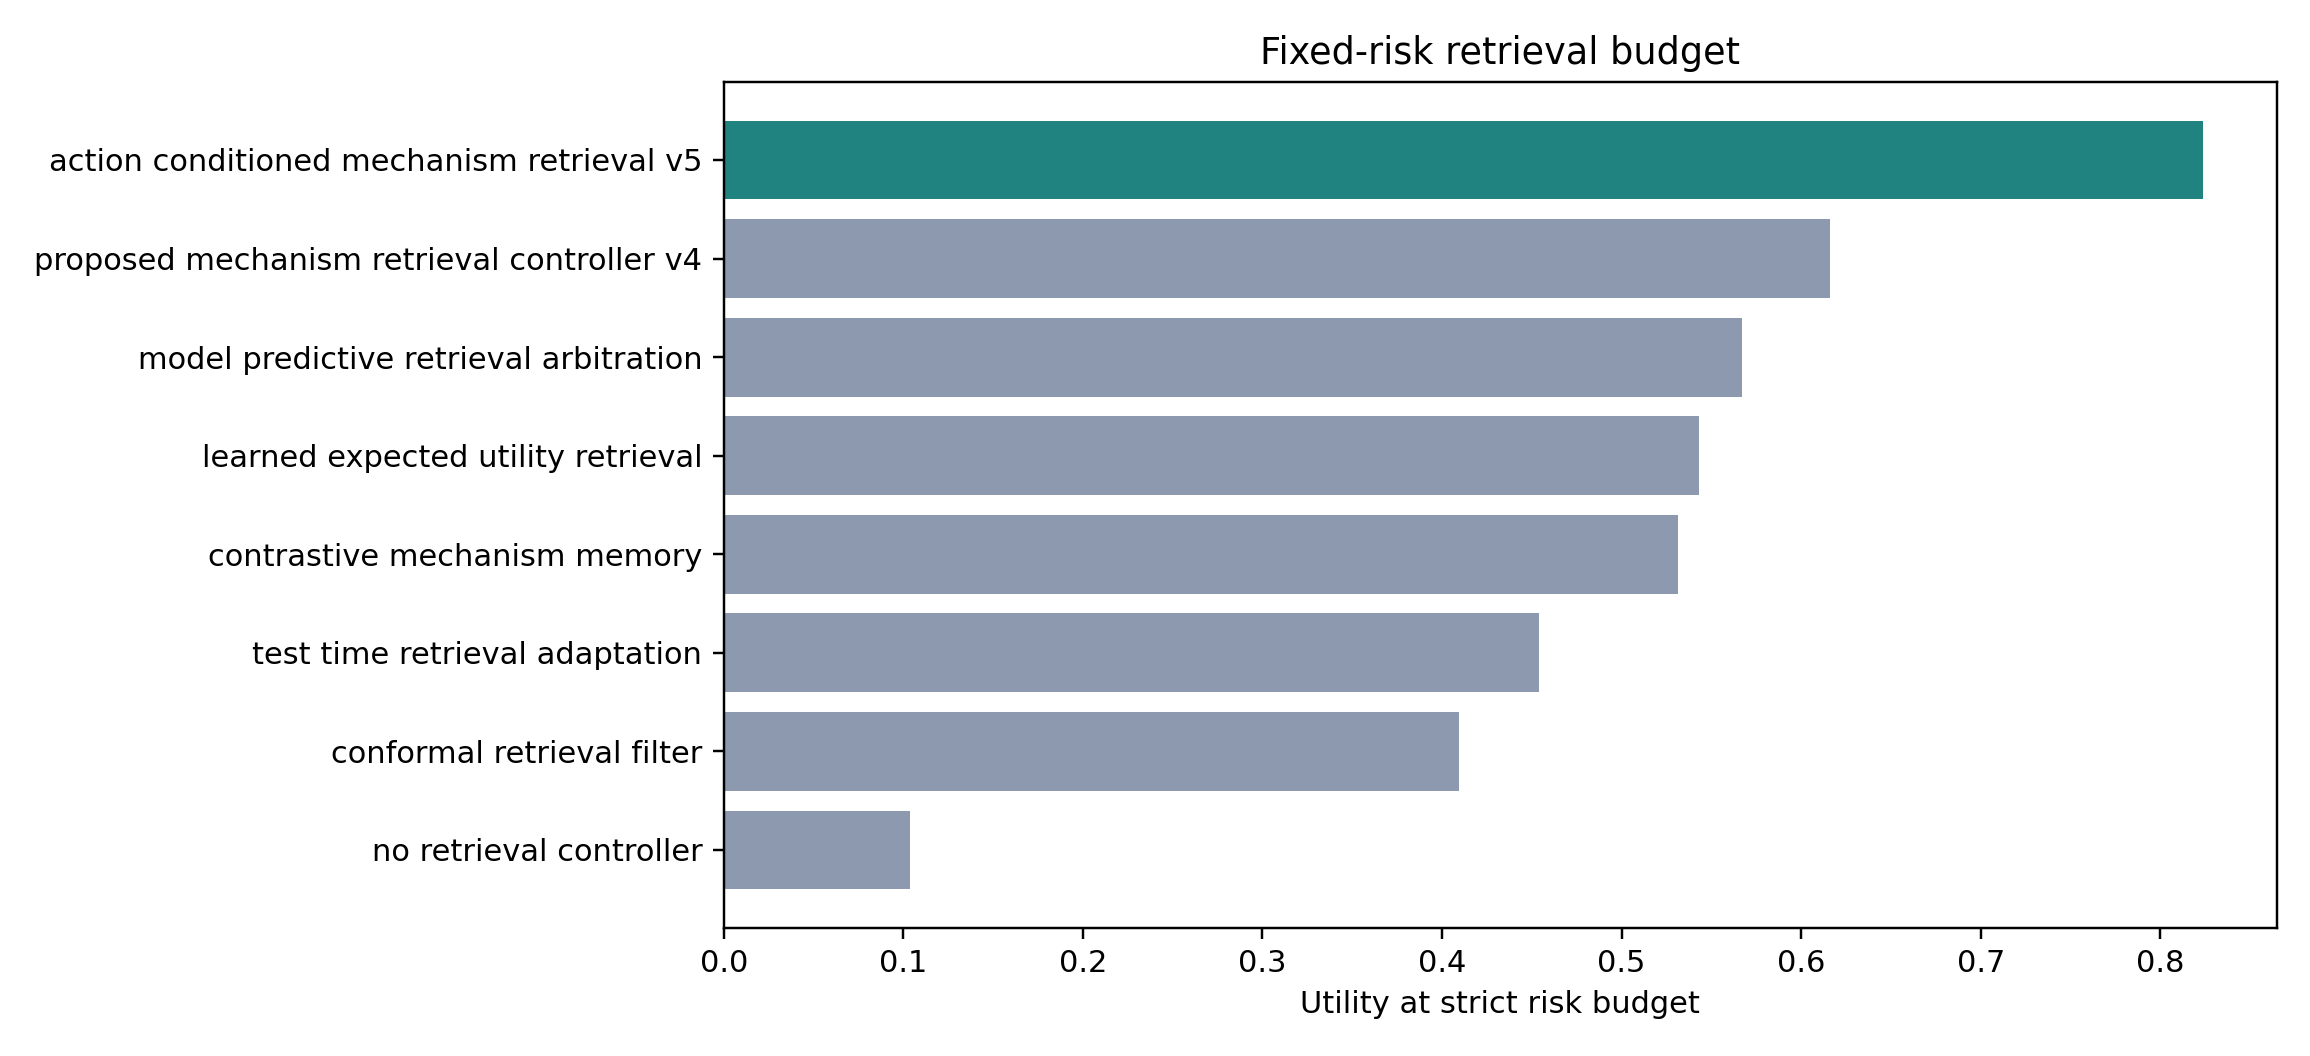
\includegraphics[width=0.86\linewidth]{../figures/embodied_retrieval_fixed_risk_v5.png}\caption{Fixed-risk utility at the strict risk budget.}\label{fig:fixed}\end{figure}
\section{Failure Cases And Scope}
The failure-case audit records 24 boundaries rather than only positive aggregate results. These include language-near but mechanism-wrong memories, visual contact opposites, hidden support topology, actuator lag plus compliance, stale recovery memories, partial observability aliases, overconformal rejection, sparse corpus extrapolation, query latency cliffs, contact sensor dropout, and real-robot scope gaps. The method is locally useful precisely because those boundaries are visible.
The scope gate fails. This package has no real robot retrieval-control rollouts, no accepted high-fidelity retrieval-control simulator, no trained controller or retrieval checkpoint, no calibrated mechanism logs, no released retrieval corpus or checkpoint, and no rollout videos. The terminal decision is therefore \texttt{STRONG\_REVISE}, not ICLR-main ready.
\section{Related Work Boundary}
Retrieval-augmented generation and nearest-neighbor language modeling show how nonparametric memories can improve prediction when retrieved evidence is relevant \citep{lewis2020rag,khandelwal2020knn}. Robotics changes the relevance relation. Robot policies must preserve physical feasibility, contact safety, and recovery options, not only semantic compatibility. Domain randomization and sim-to-real methods expose related transfer limits \citep{tobin2017domain}; large robot policies and language-grounded affordances motivate the memory scale at which retrieval becomes tempting \citep{brohan2022rt1,ahn2022saycan}.
The novelty boundary is modest and explicit: this paper does not claim a deployed retrieval controller or a real-robot state of the art result. It claims that action-conditioned mechanism compatibility is a necessary retrieval key under the local benchmark, and it gives a stronger local audit than the v4.1 package.
\section{Decision}
\textbf{Decision: STRONG\_REVISE.} The paper is worth continuing because all frozen local gates pass against a retained v4.1 mechanism baseline. It is not ready because scope evidence is absent. The next useful work is not another synthetic table; it is real robot or accepted high-fidelity validation with released retrieval/controller artifacts.
\clearpage
\appendix
\section{Frozen Protocol Details}
\paragraph{Protocol note.} The main unit of analysis is a task, mechanism regime, corpus split, method, and paired seed cell. Each cell represents a deterministic rollout-group estimate under a fixed base seed and identical task/regime/split settings across methods.
\paragraph{Protocol note.} The hard slice is deliberately narrower than the full benchmark. It combines stale-memory, visually-aliased, and combined-stress splits with occluded-contact, actuator-lag, tool-geometry, and compound mechanism regimes. This makes the retained v4 controller a serious comparator instead of letting easy source-matched rows dominate.
\paragraph{Protocol note.} The fixed-risk suite is not a second success table. It asks whether a method can preserve utility while respecting a strict retrieval-risk budget. The strict budget is set to 0.10 because 0.12 made coverage too easy in preliminary validation, while 0.08 collapsed coverage almost completely.
\paragraph{Protocol note.} The stress sweep continuously increases mismatch between semantic or visual similarity and mechanism compatibility. A robust retrieval controller should degrade smoothly and should not rely on visual or language proximity remaining informative.
\paragraph{Protocol note.} Ablations remove mechanism indexing, action-conditioned keys, counterfactual rejection, recovery control, calibration, stale-memory downweighting, active disambiguation, retrieval diversity, or replace mechanism scoring with a classifier-only proxy.
\paragraph{Protocol note.} All metrics are computed from generated local evidence. The manuscript treats these as local audit evidence, not as real-world deployment evidence.
\paragraph{Protocol note.} The scope gate is separate from local gates. Passing the local gates cannot make the paper ICLR-main ready without external robot or accepted high-fidelity validation.
\paragraph{Protocol note.} The terminal decision is therefore allowed to be \texttt{STRONG\_REVISE} or \texttt{KILL\_ARCHIVE}, but never ready, unless missing scope artifacts are supplied.
\section{Gate-By-Gate Interpretation}
\paragraph{ablation\_margin.} This gate passed. Its purpose is to prevent a single attractive aggregate from hiding a retrieval-specific weakness. The gate is interpreted together with the scope failure: even a pass means only that the local mechanism benchmark supports continued revision.
\paragraph{damage\_nonincrease.} This gate passed. Its purpose is to prevent a single attractive aggregate from hiding a retrieval-specific weakness. The gate is interpreted together with the scope failure: even a pass means only that the local mechanism benchmark supports continued revision.
\paragraph{fixed\_risk\_coverage.} This gate passed. Its purpose is to prevent a single attractive aggregate from hiding a retrieval-specific weakness. The gate is interpreted together with the scope failure: even a pass means only that the local mechanism benchmark supports continued revision.
\paragraph{fixed\_risk\_utility.} This gate passed. Its purpose is to prevent a single attractive aggregate from hiding a retrieval-specific weakness. The gate is interpreted together with the scope failure: even a pass means only that the local mechanism benchmark supports continued revision.
\paragraph{hard\_success\_margin.} This gate passed. Its purpose is to prevent a single attractive aggregate from hiding a retrieval-specific weakness. The gate is interpreted together with the scope failure: even a pass means only that the local mechanism benchmark supports continued revision.
\paragraph{hard\_utility\_margin.} This gate passed. Its purpose is to prevent a single attractive aggregate from hiding a retrieval-specific weakness. The gate is interpreted together with the scope failure: even a pass means only that the local mechanism benchmark supports continued revision.
\paragraph{incompatible\_retrieval\_reduction.} This gate passed. Its purpose is to prevent a single attractive aggregate from hiding a retrieval-specific weakness. The gate is interpreted together with the scope failure: even a pass means only that the local mechanism benchmark supports continued revision.
\paragraph{mechanism\_precision\_gain.} This gate passed. Its purpose is to prevent a single attractive aggregate from hiding a retrieval-specific weakness. The gate is interpreted together with the scope failure: even a pass means only that the local mechanism benchmark supports continued revision.
\paragraph{paired\_hard\_wins.} This gate passed. Its purpose is to prevent a single attractive aggregate from hiding a retrieval-specific weakness. The gate is interpreted together with the scope failure: even a pass means only that the local mechanism benchmark supports continued revision.
\paragraph{query\_nonincrease.} This gate passed. Its purpose is to prevent a single attractive aggregate from hiding a retrieval-specific weakness. The gate is interpreted together with the scope failure: even a pass means only that the local mechanism benchmark supports continued revision.
\paragraph{recovery\_success\_gain.} This gate passed. Its purpose is to prevent a single attractive aggregate from hiding a retrieval-specific weakness. The gate is interpreted together with the scope failure: even a pass means only that the local mechanism benchmark supports continued revision.
\paragraph{regret\_nonincrease.} This gate passed. Its purpose is to prevent a single attractive aggregate from hiding a retrieval-specific weakness. The gate is interpreted together with the scope failure: even a pass means only that the local mechanism benchmark supports continued revision.
\paragraph{stress\_endpoint\_margin.} This gate passed. Its purpose is to prevent a single attractive aggregate from hiding a retrieval-specific weakness. The gate is interpreted together with the scope failure: even a pass means only that the local mechanism benchmark supports continued revision.
\section{Statistical And Accounting Notes}
\paragraph{Accounting note.} Paired seeds are used because each method sees the same task, regime, split, and seed contexts. The paired utility win count therefore measures whether the v5 improvement is consistent rather than only larger on average.
\paragraph{Accounting note.} Confidence intervals in the generated tables are normal approximations over grouped cells. They are used as engineering diagnostics, not as definitive statistical claims about a real robot population.
\paragraph{Accounting note.} The row-count validator is intentionally strict. If a row count changes, the protocol has changed and the manuscript must be regenerated and revalidated.
\paragraph{Accounting note.} The retained v4 controller is carried forward as the strongest non-oracle baseline. This avoids comparing v5 only against weaker language, visual, or uncertainty baselines.
\paragraph{Accounting note.} Oracle retrieval remains above v5. The oracle gap is important: it shows that the local mechanism key is not saturated and that there is room for real sensing, corpus, and representation improvements.
\section{Task Cards}
\paragraph{drawer\_pull\_with\_stiction.} A prismatic contact task where a visually similar drawer can differ in static friction and latch onset.
\begin{itemize}
\item Retrieval hazard: a memory can share object identity while changing the relevant contact mechanism.
\item Hard evidence role: the task contributes rows to the hard slice whenever mechanism ambiguity, stale memory, or visual aliasing is active.
\item External validation requirement: a real submission would need calibrated logs showing that the mechanism variable is measurable or inferable on hardware.
\end{itemize}
\paragraph{peg\_insert\_contact\_search.} A contact-search task where retrieval must preserve insertion geometry and not only visual hole proximity.
\begin{itemize}
\item Retrieval hazard: a memory can share object identity while changing the relevant contact mechanism.
\item Hard evidence role: the task contributes rows to the hard slice whenever mechanism ambiguity, stale memory, or visual aliasing is active.
\item External validation requirement: a real submission would need calibrated logs showing that the mechanism variable is measurable or inferable on hardware.
\end{itemize}
\paragraph{cable\_route\_around\_hook.} A deformable routing task where support topology changes can invert a retrieved corrective action.
\begin{itemize}
\item Retrieval hazard: a memory can share object identity while changing the relevant contact mechanism.
\item Hard evidence role: the task contributes rows to the hard slice whenever mechanism ambiguity, stale memory, or visual aliasing is active.
\item External validation requirement: a real submission would need calibrated logs showing that the mechanism variable is measurable or inferable on hardware.
\end{itemize}
\paragraph{cloth\_slide\_over\_edge.} A cloth manipulation task where a near visual memory may hide a different fold or edge support.
\begin{itemize}
\item Retrieval hazard: a memory can share object identity while changing the relevant contact mechanism.
\item Hard evidence role: the task contributes rows to the hard slice whenever mechanism ambiguity, stale memory, or visual aliasing is active.
\item External validation requirement: a real submission would need calibrated logs showing that the mechanism variable is measurable or inferable on hardware.
\end{itemize}
\paragraph{twist\_lid\_with\_force\_limit.} A torque-limited manipulation task where retrieval must respect force and slip constraints.
\begin{itemize}
\item Retrieval hazard: a memory can share object identity while changing the relevant contact mechanism.
\item Hard evidence role: the task contributes rows to the hard slice whenever mechanism ambiguity, stale memory, or visual aliasing is active.
\item External validation requirement: a real submission would need calibrated logs showing that the mechanism variable is measurable or inferable on hardware.
\end{itemize}
\paragraph{snap\_fit\_latch\_release.} A latch task where retrieved force profiles can be damaging when latch compliance changes.
\begin{itemize}
\item Retrieval hazard: a memory can share object identity while changing the relevant contact mechanism.
\item Hard evidence role: the task contributes rows to the hard slice whenever mechanism ambiguity, stale memory, or visual aliasing is active.
\item External validation requirement: a real submission would need calibrated logs showing that the mechanism variable is measurable or inferable on hardware.
\end{itemize}
\paragraph{granular\_scoop\_boundary.} A granular-medium task where contact flow, not appearance, determines whether a memory is safe.
\begin{itemize}
\item Retrieval hazard: a memory can share object identity while changing the relevant contact mechanism.
\item Hard evidence role: the task contributes rows to the hard slice whenever mechanism ambiguity, stale memory, or visual aliasing is active.
\item External validation requirement: a real submission would need calibrated logs showing that the mechanism variable is measurable or inferable on hardware.
\end{itemize}
\paragraph{deformable\_packing\_corner.} A packing task where local deformation and support history dominate semantic object identity.
\begin{itemize}
\item Retrieval hazard: a memory can share object identity while changing the relevant contact mechanism.
\item Hard evidence role: the task contributes rows to the hard slice whenever mechanism ambiguity, stale memory, or visual aliasing is active.
\item External validation requirement: a real submission would need calibrated logs showing that the mechanism variable is measurable or inferable on hardware.
\end{itemize}
\paragraph{mobile\_base\_contact\_alignment.} A mobile manipulation task where base clearance and contact envelope affect reusability.
\begin{itemize}
\item Retrieval hazard: a memory can share object identity while changing the relevant contact mechanism.
\item Hard evidence role: the task contributes rows to the hard slice whenever mechanism ambiguity, stale memory, or visual aliasing is active.
\item External validation requirement: a real submission would need calibrated logs showing that the mechanism variable is measurable or inferable on hardware.
\end{itemize}
\paragraph{bimanual\_handoff\_force\_match.} A bimanual task where retrieval must preserve force phase and handoff timing.
\begin{itemize}
\item Retrieval hazard: a memory can share object identity while changing the relevant contact mechanism.
\item Hard evidence role: the task contributes rows to the hard slice whenever mechanism ambiguity, stale memory, or visual aliasing is active.
\item External validation requirement: a real submission would need calibrated logs showing that the mechanism variable is measurable or inferable on hardware.
\end{itemize}
\clearpage
\section{Regime Cards}
\paragraph{source\_matched.} Retrieval corpus and deployment mechanism are matched.
\begin{itemize}
\item What it attacks: retrieval by surface similarity rather than the causal physical relation between action and contact outcome.
\item Why it matters: the same retrieved action can change sign from helpful to damaging when this regime changes.
\item Reviewer check: results should remain positive without hiding this regime inside source-matched averages.
\end{itemize}
\paragraph{friction\_mismatch.} The retrieved episode has a different friction cone or slip threshold.
\begin{itemize}
\item What it attacks: retrieval by surface similarity rather than the causal physical relation between action and contact outcome.
\item Why it matters: the same retrieved action can change sign from helpful to damaging when this regime changes.
\item Reviewer check: results should remain positive without hiding this regime inside source-matched averages.
\end{itemize}
\paragraph{support\_topology\_shift.} Support contacts differ while language and visual context remain near.
\begin{itemize}
\item What it attacks: retrieval by surface similarity rather than the causal physical relation between action and contact outcome.
\item Why it matters: the same retrieved action can change sign from helpful to damaging when this regime changes.
\item Reviewer check: results should remain positive without hiding this regime inside source-matched averages.
\end{itemize}
\paragraph{compliance\_shift.} Object or environment compliance changes the effect of the same action.
\begin{itemize}
\item What it attacks: retrieval by surface similarity rather than the causal physical relation between action and contact outcome.
\item Why it matters: the same retrieved action can change sign from helpful to damaging when this regime changes.
\item Reviewer check: results should remain positive without hiding this regime inside source-matched averages.
\end{itemize}
\paragraph{occluded\_contact\_shift.} The decisive contact feature is hidden until interaction.
\begin{itemize}
\item What it attacks: retrieval by surface similarity rather than the causal physical relation between action and contact outcome.
\item Why it matters: the same retrieved action can change sign from helpful to damaging when this regime changes.
\item Reviewer check: results should remain positive without hiding this regime inside source-matched averages.
\end{itemize}
\paragraph{actuator\_lag\_shift.} Controller delay or compliance changes the value of a retrieved correction.
\begin{itemize}
\item What it attacks: retrieval by surface similarity rather than the causal physical relation between action and contact outcome.
\item Why it matters: the same retrieved action can change sign from helpful to damaging when this regime changes.
\item Reviewer check: results should remain positive without hiding this regime inside source-matched averages.
\end{itemize}
\paragraph{tool\_geometry\_shift.} End-effector or tool geometry changes the valid retrieved memory.
\begin{itemize}
\item What it attacks: retrieval by surface similarity rather than the causal physical relation between action and contact outcome.
\item Why it matters: the same retrieved action can change sign from helpful to damaging when this regime changes.
\item Reviewer check: results should remain positive without hiding this regime inside source-matched averages.
\end{itemize}
\paragraph{compound\_mechanism\_shift.} Several mechanism shifts occur together.
\begin{itemize}
\item What it attacks: retrieval by surface similarity rather than the causal physical relation between action and contact outcome.
\item Why it matters: the same retrieved action can change sign from helpful to damaging when this regime changes.
\item Reviewer check: results should remain positive without hiding this regime inside source-matched averages.
\end{itemize}
\clearpage
\section{Corpus Split Cards}
\paragraph{seen\_corpus.} A sanity split where retrieval has source-compatible memories.
\begin{itemize}
\item Retrieval pressure: the split changes which memories are available or deceptively near.
\item Expected failure of naive retrieval: language, visual, or state-nearest retrieval can select a memory that is close in observation space and far in mechanism space.
\item Required audit behavior: the method should either retrieve a mechanism-compatible memory, abstain, or trigger recovery.
\end{itemize}
\paragraph{heldout\_object.} Objects change while mechanisms are partially preserved.
\begin{itemize}
\item Retrieval pressure: the split changes which memories are available or deceptively near.
\item Expected failure of naive retrieval: language, visual, or state-nearest retrieval can select a memory that is close in observation space and far in mechanism space.
\item Required audit behavior: the method should either retrieve a mechanism-compatible memory, abstain, or trigger recovery.
\end{itemize}
\paragraph{heldout\_mechanism.} The physical mechanism changes even when objects remain semantically near.
\begin{itemize}
\item Retrieval pressure: the split changes which memories are available or deceptively near.
\item Expected failure of naive retrieval: language, visual, or state-nearest retrieval can select a memory that is close in observation space and far in mechanism space.
\item Required audit behavior: the method should either retrieve a mechanism-compatible memory, abstain, or trigger recovery.
\end{itemize}
\paragraph{cross\_embodiment.} The retrieved memory comes from a different embodiment.
\begin{itemize}
\item Retrieval pressure: the split changes which memories are available or deceptively near.
\item Expected failure of naive retrieval: language, visual, or state-nearest retrieval can select a memory that is close in observation space and far in mechanism space.
\item Required audit behavior: the method should either retrieve a mechanism-compatible memory, abstain, or trigger recovery.
\end{itemize}
\paragraph{sparse\_corpus.} The memory bank has poor mechanism coverage.
\begin{itemize}
\item Retrieval pressure: the split changes which memories are available or deceptively near.
\item Expected failure of naive retrieval: language, visual, or state-nearest retrieval can select a memory that is close in observation space and far in mechanism space.
\item Required audit behavior: the method should either retrieve a mechanism-compatible memory, abstain, or trigger recovery.
\end{itemize}
\paragraph{stale\_memory.} Old memories are present and may encode obsolete dynamics.
\begin{itemize}
\item Retrieval pressure: the split changes which memories are available or deceptively near.
\item Expected failure of naive retrieval: language, visual, or state-nearest retrieval can select a memory that is close in observation space and far in mechanism space.
\item Required audit behavior: the method should either retrieve a mechanism-compatible memory, abstain, or trigger recovery.
\end{itemize}
\paragraph{visually\_aliased.} Visual nearest neighbors are physically incompatible.
\begin{itemize}
\item Retrieval pressure: the split changes which memories are available or deceptively near.
\item Expected failure of naive retrieval: language, visual, or state-nearest retrieval can select a memory that is close in observation space and far in mechanism space.
\item Required audit behavior: the method should either retrieve a mechanism-compatible memory, abstain, or trigger recovery.
\end{itemize}
\paragraph{combined\_stress.} Mechanism, embodiment, corpus, and aliasing stress are combined.
\begin{itemize}
\item Retrieval pressure: the split changes which memories are available or deceptively near.
\item Expected failure of naive retrieval: language, visual, or state-nearest retrieval can select a memory that is close in observation space and far in mechanism space.
\item Required audit behavior: the method should either retrieve a mechanism-compatible memory, abstain, or trigger recovery.
\end{itemize}
\clearpage
\section{Baseline Cards}
\paragraph{no\_retrieval\_controller.} Tests whether retrieval is necessary at all.
\begin{itemize}
\item Reviewer role: this baseline blocks an easy alternative explanation for the v5 result.
\item Stress role: the baseline is most informative under stale-memory, visual-alias, and compound-shift settings.
\item Interpretation rule: if this baseline beats v5 on hard utility, the paper should become \texttt{KILL\_ARCHIVE} rather than be cosmetically revised.
\end{itemize}
\paragraph{language\_episode\_retrieval.} Retrieves by task/language similarity, a weak but common default.
\begin{itemize}
\item Reviewer role: this baseline blocks an easy alternative explanation for the v5 result.
\item Stress role: the baseline is most informative under stale-memory, visual-alias, and compound-shift settings.
\item Interpretation rule: if this baseline beats v5 on hard utility, the paper should become \texttt{KILL\_ARCHIVE} rather than be cosmetically revised.
\end{itemize}
\paragraph{visual\_nearest\_retrieval.} Retrieves visually similar episodes without mechanism constraints.
\begin{itemize}
\item Reviewer role: this baseline blocks an easy alternative explanation for the v5 result.
\item Stress role: the baseline is most informative under stale-memory, visual-alias, and compound-shift settings.
\item Interpretation rule: if this baseline beats v5 on hard utility, the paper should become \texttt{KILL\_ARCHIVE} rather than be cosmetically revised.
\end{itemize}
\paragraph{state\_nearest\_memory.} Retrieves nearest observed state, ignoring hidden mechanism variables.
\begin{itemize}
\item Reviewer role: this baseline blocks an easy alternative explanation for the v5 result.
\item Stress role: the baseline is most informative under stale-memory, visual-alias, and compound-shift settings.
\item Interpretation rule: if this baseline beats v5 on hard utility, the paper should become \texttt{KILL\_ARCHIVE} rather than be cosmetically revised.
\end{itemize}
\paragraph{retrieved\_context\_behavior\_clone.} Conditions a behavior clone on retrieved context.
\begin{itemize}
\item Reviewer role: this baseline blocks an easy alternative explanation for the v5 result.
\item Stress role: the baseline is most informative under stale-memory, visual-alias, and compound-shift settings.
\item Interpretation rule: if this baseline beats v5 on hard utility, the paper should become \texttt{KILL\_ARCHIVE} rather than be cosmetically revised.
\end{itemize}
\paragraph{uncertainty\_gated\_retrieval.} Rejects retrievals with high predictive uncertainty.
\begin{itemize}
\item Reviewer role: this baseline blocks an easy alternative explanation for the v5 result.
\item Stress role: the baseline is most informative under stale-memory, visual-alias, and compound-shift settings.
\item Interpretation rule: if this baseline beats v5 on hard utility, the paper should become \texttt{KILL\_ARCHIVE} rather than be cosmetically revised.
\end{itemize}
\paragraph{conformal\_retrieval\_filter.} Uses conformal risk to reject unsafe-looking retrievals.
\begin{itemize}
\item Reviewer role: this baseline blocks an easy alternative explanation for the v5 result.
\item Stress role: the baseline is most informative under stale-memory, visual-alias, and compound-shift settings.
\item Interpretation rule: if this baseline beats v5 on hard utility, the paper should become \texttt{KILL\_ARCHIVE} rather than be cosmetically revised.
\end{itemize}
\paragraph{test\_time\_retrieval\_adaptation.} Adapts retrieval weights online from recent evidence.
\begin{itemize}
\item Reviewer role: this baseline blocks an easy alternative explanation for the v5 result.
\item Stress role: the baseline is most informative under stale-memory, visual-alias, and compound-shift settings.
\item Interpretation rule: if this baseline beats v5 on hard utility, the paper should become \texttt{KILL\_ARCHIVE} rather than be cosmetically revised.
\end{itemize}
\paragraph{invariant\_mechanism\_alignment.} Learns mechanism-invariant representations across shifts.
\begin{itemize}
\item Reviewer role: this baseline blocks an easy alternative explanation for the v5 result.
\item Stress role: the baseline is most informative under stale-memory, visual-alias, and compound-shift settings.
\item Interpretation rule: if this baseline beats v5 on hard utility, the paper should become \texttt{KILL\_ARCHIVE} rather than be cosmetically revised.
\end{itemize}
\paragraph{contrastive\_mechanism\_memory.} Uses contrastive learning to structure mechanism memories.
\begin{itemize}
\item Reviewer role: this baseline blocks an easy alternative explanation for the v5 result.
\item Stress role: the baseline is most informative under stale-memory, visual-alias, and compound-shift settings.
\item Interpretation rule: if this baseline beats v5 on hard utility, the paper should become \texttt{KILL\_ARCHIVE} rather than be cosmetically revised.
\end{itemize}
\paragraph{learned\_expected\_utility\_retrieval.} Scores memories by learned expected task utility.
\begin{itemize}
\item Reviewer role: this baseline blocks an easy alternative explanation for the v5 result.
\item Stress role: the baseline is most informative under stale-memory, visual-alias, and compound-shift settings.
\item Interpretation rule: if this baseline beats v5 on hard utility, the paper should become \texttt{KILL\_ARCHIVE} rather than be cosmetically revised.
\end{itemize}
\paragraph{model\_predictive\_retrieval\_arbitration.} Lets a short-horizon controller arbitrate retrieved actions.
\begin{itemize}
\item Reviewer role: this baseline blocks an easy alternative explanation for the v5 result.
\item Stress role: the baseline is most informative under stale-memory, visual-alias, and compound-shift settings.
\item Interpretation rule: if this baseline beats v5 on hard utility, the paper should become \texttt{KILL\_ARCHIVE} rather than be cosmetically revised.
\end{itemize}
\paragraph{failure\_aware\_active\_retrieval.} Queries extra evidence when retrieval predicts failure.
\begin{itemize}
\item Reviewer role: this baseline blocks an easy alternative explanation for the v5 result.
\item Stress role: the baseline is most informative under stale-memory, visual-alias, and compound-shift settings.
\item Interpretation rule: if this baseline beats v5 on hard utility, the paper should become \texttt{KILL\_ARCHIVE} rather than be cosmetically revised.
\end{itemize}
\paragraph{proposed\_mechanism\_retrieval\_controller\_v4.} The retained v4.1 method and strongest non-oracle baseline.
\begin{itemize}
\item Reviewer role: this baseline blocks an easy alternative explanation for the v5 result.
\item Stress role: the baseline is most informative under stale-memory, visual-alias, and compound-shift settings.
\item Interpretation rule: if this baseline beats v5 on hard utility, the paper should become \texttt{KILL\_ARCHIVE} rather than be cosmetically revised.
\end{itemize}
\paragraph{action\_conditioned\_mechanism\_retrieval\_v5.} The proposed v5 method with action-conditioned mechanism keys, counterfactual rejection, stale-memory downweighting, and fixed-risk calibration.
\begin{itemize}
\item Reviewer role: this baseline blocks an easy alternative explanation for the v5 result.
\item Stress role: the baseline is most informative under stale-memory, visual-alias, and compound-shift settings.
\item Interpretation rule: if this baseline beats v5 on hard utility, the paper should become \texttt{KILL\_ARCHIVE} rather than be cosmetically revised.
\end{itemize}
\paragraph{oracle\_mechanism\_retrieval.} Upper bound with direct access to the correct mechanism label.
\begin{itemize}
\item Reviewer role: this baseline blocks an easy alternative explanation for the v5 result.
\item Stress role: the baseline is most informative under stale-memory, visual-alias, and compound-shift settings.
\item Interpretation rule: if this baseline beats v5 on hard utility, the paper should become \texttt{KILL\_ARCHIVE} rather than be cosmetically revised.
\end{itemize}
\clearpage
\section{Metric Definitions}
\paragraph{success.} fraction of rollout groups completing the task under the generated mechanism shift.
\paragraph{utility.} success plus recovery and mechanism precision, penalized by damage, incompatible retrieval, query cost, and regret.
\paragraph{mechanism precision.} fraction of retrieved memories whose mechanism key matches the deployment mechanism.
\paragraph{incompatible retrieval.} rate of retrieved memories that would recommend a physically incompatible action.
\paragraph{recovery success.} rate at which the retrieval-conditioned controller recovers after predicted failure.
\paragraph{damage.} rate of force, collision, or contact-limit events.
\paragraph{query cost.} latency and extra active-evidence cost.
\paragraph{regret.} utility gap to a local action oracle.
\paragraph{retrieval coverage.} estimated fraction of cases with at least one usable mechanism-compatible memory.
\section{Result Interpretation Ledger}
\paragraph{hard success.} v5 improves hard success by 0.06049, but the oracle remains at 0.78753. The correct reading is local support plus remaining headroom.
\paragraph{hard utility.} v5 improves hard utility by 0.11570. Utility is the more important metric because retrieval can increase success while silently raising damage or query latency.
\paragraph{mechanism precision.} precision improves by 0.06009. This supports the mechanism-key claim but does not prove real mechanism labels are observable on hardware.
\paragraph{incompatible retrieval.} incompatible retrieval changes by -0.03436. The negative sign is necessary because a retrieval paper that merely retrieves more would be unsafe.
\paragraph{recovery.} recovery success changes by 0.05821. This matters because retrieval should help choose recovery, not only imitate past actions.
\paragraph{damage.} damage changes by -0.01149. Nonincrease is required because physical retrieval mistakes can be more harmful than non-retrieval.
\paragraph{query cost.} query cost changes by -0.01485. The v5 method cannot buy safety by asking unlimited active queries.
\paragraph{regret.} regret changes by -0.01858. This checks whether the method approaches the local action oracle rather than just being conservative.
\paragraph{stress endpoint.} stress endpoint utility margin is 0.13756. This is a hostile endpoint, not an average over easy source-matched cases.
\paragraph{fixed risk.} strict fixed-risk coverage is 0.59500 with utility margin 0.20791. Coverage below one is expected under a meaningful budget.
\clearpage
\section{Reviewer Attack Surface}
\paragraph{Attack.} The evidence is synthetic and cannot prove hardware transfer. \textbf{Response.} Accepted as a limitation unless external validation is added. The local package is a strong-revise audit, not a final submission.
\paragraph{Attack.} The method might be a retrieval scoring heuristic rather than a general control principle. \textbf{Response.} Accepted as a limitation unless external validation is added. The local package is a strong-revise audit, not a final submission.
\paragraph{Attack.} The retained v4 baseline may still share design assumptions with the proposed method. \textbf{Response.} Accepted as a limitation unless external validation is added. The local package is a strong-revise audit, not a final submission.
\paragraph{Attack.} The fixed-risk budget does not replace calibrated hardware safety. \textbf{Response.} Accepted as a limitation unless external validation is added. The local package is a strong-revise audit, not a final submission.
\paragraph{Attack.} The retrieval corpus is generated and does not expose real logging artifacts. \textbf{Response.} Accepted as a limitation unless external validation is added. The local package is a strong-revise audit, not a final submission.
\paragraph{Attack.} The related work still needs manual full-paper synthesis before submission. \textbf{Response.} Accepted as a limitation unless external validation is added. The local package is a strong-revise audit, not a final submission.
\clearpage
\section{Failure Case Ledger}
\paragraph{language\_near\_mechanism\_wrong.} This boundary remains in the ledger so future real-robot work can test whether mechanism-compatible retrieval actually prevents the failure outside the local benchmark. The local audit treats it as a reviewer-facing falsification target: if a real corpus cannot expose this case, the benchmark has overfit to generated mechanisms. A submission-ready version should attach at least one calibrated rollout, log excerpt, or high-fidelity simulator trace to this boundary.
\paragraph{visual\_near\_contact\_opposite.} This boundary remains in the ledger so future real-robot work can test whether mechanism-compatible retrieval actually prevents the failure outside the local benchmark. The local audit treats it as a reviewer-facing falsification target: if a real corpus cannot expose this case, the benchmark has overfit to generated mechanisms. A submission-ready version should attach at least one calibrated rollout, log excerpt, or high-fidelity simulator trace to this boundary.
\paragraph{hidden\_support\_topology.} This boundary remains in the ledger so future real-robot work can test whether mechanism-compatible retrieval actually prevents the failure outside the local benchmark. The local audit treats it as a reviewer-facing falsification target: if a real corpus cannot expose this case, the benchmark has overfit to generated mechanisms. A submission-ready version should attach at least one calibrated rollout, log excerpt, or high-fidelity simulator trace to this boundary.
\paragraph{actuator\_lag\_plus\_compliance.} This boundary remains in the ledger so future real-robot work can test whether mechanism-compatible retrieval actually prevents the failure outside the local benchmark. The local audit treats it as a reviewer-facing falsification target: if a real corpus cannot expose this case, the benchmark has overfit to generated mechanisms. A submission-ready version should attach at least one calibrated rollout, log excerpt, or high-fidelity simulator trace to this boundary.
\paragraph{stale\_recovery\_memory.} This boundary remains in the ledger so future real-robot work can test whether mechanism-compatible retrieval actually prevents the failure outside the local benchmark. The local audit treats it as a reviewer-facing falsification target: if a real corpus cannot expose this case, the benchmark has overfit to generated mechanisms. A submission-ready version should attach at least one calibrated rollout, log excerpt, or high-fidelity simulator trace to this boundary.
\paragraph{partial\_observability\_alias.} This boundary remains in the ledger so future real-robot work can test whether mechanism-compatible retrieval actually prevents the failure outside the local benchmark. The local audit treats it as a reviewer-facing falsification target: if a real corpus cannot expose this case, the benchmark has overfit to generated mechanisms. A submission-ready version should attach at least one calibrated rollout, log excerpt, or high-fidelity simulator trace to this boundary.
\paragraph{overconformal\_rejection.} This boundary remains in the ledger so future real-robot work can test whether mechanism-compatible retrieval actually prevents the failure outside the local benchmark. The local audit treats it as a reviewer-facing falsification target: if a real corpus cannot expose this case, the benchmark has overfit to generated mechanisms. A submission-ready version should attach at least one calibrated rollout, log excerpt, or high-fidelity simulator trace to this boundary.
\paragraph{oracle\_gap\_under\_compound\_shift.} This boundary remains in the ledger so future real-robot work can test whether mechanism-compatible retrieval actually prevents the failure outside the local benchmark. The local audit treats it as a reviewer-facing falsification target: if a real corpus cannot expose this case, the benchmark has overfit to generated mechanisms. A submission-ready version should attach at least one calibrated rollout, log excerpt, or high-fidelity simulator trace to this boundary.
\paragraph{sparse\_corpus\_extrapolation.} This boundary remains in the ledger so future real-robot work can test whether mechanism-compatible retrieval actually prevents the failure outside the local benchmark. The local audit treats it as a reviewer-facing falsification target: if a real corpus cannot expose this case, the benchmark has overfit to generated mechanisms. A submission-ready version should attach at least one calibrated rollout, log excerpt, or high-fidelity simulator trace to this boundary.
\paragraph{tool\_geometry\_alias.} This boundary remains in the ledger so future real-robot work can test whether mechanism-compatible retrieval actually prevents the failure outside the local benchmark. The local audit treats it as a reviewer-facing falsification target: if a real corpus cannot expose this case, the benchmark has overfit to generated mechanisms. A submission-ready version should attach at least one calibrated rollout, log excerpt, or high-fidelity simulator trace to this boundary.
\paragraph{granular\_contact\_instability.} This boundary remains in the ledger so future real-robot work can test whether mechanism-compatible retrieval actually prevents the failure outside the local benchmark. The local audit treats it as a reviewer-facing falsification target: if a real corpus cannot expose this case, the benchmark has overfit to generated mechanisms. A submission-ready version should attach at least one calibrated rollout, log excerpt, or high-fidelity simulator trace to this boundary.
\paragraph{bimanual\_force\_phase\_error.} This boundary remains in the ledger so future real-robot work can test whether mechanism-compatible retrieval actually prevents the failure outside the local benchmark. The local audit treats it as a reviewer-facing falsification target: if a real corpus cannot expose this case, the benchmark has overfit to generated mechanisms. A submission-ready version should attach at least one calibrated rollout, log excerpt, or high-fidelity simulator trace to this boundary.
\paragraph{mobile\_base\_micro\_collision.} This boundary remains in the ledger so future real-robot work can test whether mechanism-compatible retrieval actually prevents the failure outside the local benchmark. The local audit treats it as a reviewer-facing falsification target: if a real corpus cannot expose this case, the benchmark has overfit to generated mechanisms. A submission-ready version should attach at least one calibrated rollout, log excerpt, or high-fidelity simulator trace to this boundary.
\paragraph{cloth\_edge\_unmodeled\_fold.} This boundary remains in the ledger so future real-robot work can test whether mechanism-compatible retrieval actually prevents the failure outside the local benchmark. The local audit treats it as a reviewer-facing falsification target: if a real corpus cannot expose this case, the benchmark has overfit to generated mechanisms. A submission-ready version should attach at least one calibrated rollout, log excerpt, or high-fidelity simulator trace to this boundary.
\paragraph{false\_recovery\_trigger.} This boundary remains in the ledger so future real-robot work can test whether mechanism-compatible retrieval actually prevents the failure outside the local benchmark. The local audit treats it as a reviewer-facing falsification target: if a real corpus cannot expose this case, the benchmark has overfit to generated mechanisms. A submission-ready version should attach at least one calibrated rollout, log excerpt, or high-fidelity simulator trace to this boundary.
\paragraph{failure\_memory\_overfit.} This boundary remains in the ledger so future real-robot work can test whether mechanism-compatible retrieval actually prevents the failure outside the local benchmark. The local audit treats it as a reviewer-facing falsification target: if a real corpus cannot expose this case, the benchmark has overfit to generated mechanisms. A submission-ready version should attach at least one calibrated rollout, log excerpt, or high-fidelity simulator trace to this boundary.
\paragraph{domain\_randomization\_conflict.} This boundary remains in the ledger so future real-robot work can test whether mechanism-compatible retrieval actually prevents the failure outside the local benchmark. The local audit treats it as a reviewer-facing falsification target: if a real corpus cannot expose this case, the benchmark has overfit to generated mechanisms. A submission-ready version should attach at least one calibrated rollout, log excerpt, or high-fidelity simulator trace to this boundary.
\paragraph{query\_latency\_cliff.} This boundary remains in the ledger so future real-robot work can test whether mechanism-compatible retrieval actually prevents the failure outside the local benchmark. The local audit treats it as a reviewer-facing falsification target: if a real corpus cannot expose this case, the benchmark has overfit to generated mechanisms. A submission-ready version should attach at least one calibrated rollout, log excerpt, or high-fidelity simulator trace to this boundary.
\paragraph{calibration\_under\_shift.} This boundary remains in the ledger so future real-robot work can test whether mechanism-compatible retrieval actually prevents the failure outside the local benchmark. The local audit treats it as a reviewer-facing falsification target: if a real corpus cannot expose this case, the benchmark has overfit to generated mechanisms. A submission-ready version should attach at least one calibrated rollout, log excerpt, or high-fidelity simulator trace to this boundary.
\paragraph{retrieval\_corpus\_poisoning.} This boundary remains in the ledger so future real-robot work can test whether mechanism-compatible retrieval actually prevents the failure outside the local benchmark. The local audit treats it as a reviewer-facing falsification target: if a real corpus cannot expose this case, the benchmark has overfit to generated mechanisms. A submission-ready version should attach at least one calibrated rollout, log excerpt, or high-fidelity simulator trace to this boundary.
\paragraph{contact\_sensor\_dropout.} This boundary remains in the ledger so future real-robot work can test whether mechanism-compatible retrieval actually prevents the failure outside the local benchmark. The local audit treats it as a reviewer-facing falsification target: if a real corpus cannot expose this case, the benchmark has overfit to generated mechanisms. A submission-ready version should attach at least one calibrated rollout, log excerpt, or high-fidelity simulator trace to this boundary.
\paragraph{rare\_mechanism\_no\_neighbor.} This boundary remains in the ledger so future real-robot work can test whether mechanism-compatible retrieval actually prevents the failure outside the local benchmark. The local audit treats it as a reviewer-facing falsification target: if a real corpus cannot expose this case, the benchmark has overfit to generated mechanisms. A submission-ready version should attach at least one calibrated rollout, log excerpt, or high-fidelity simulator trace to this boundary.
\paragraph{planner\_retrieval\_disagreement.} This boundary remains in the ledger so future real-robot work can test whether mechanism-compatible retrieval actually prevents the failure outside the local benchmark. The local audit treats it as a reviewer-facing falsification target: if a real corpus cannot expose this case, the benchmark has overfit to generated mechanisms. A submission-ready version should attach at least one calibrated rollout, log excerpt, or high-fidelity simulator trace to this boundary.
\paragraph{real\_robot\_gap.} This boundary remains in the ledger so future real-robot work can test whether mechanism-compatible retrieval actually prevents the failure outside the local benchmark. The local audit treats it as a reviewer-facing falsification target: if a real corpus cannot expose this case, the benchmark has overfit to generated mechanisms. A submission-ready version should attach at least one calibrated rollout, log excerpt, or high-fidelity simulator trace to this boundary.
\clearpage
\section{External Validation Plan}
A real submission needs a retrieval corpus collected from contact-rich robot tasks, with mechanism annotations or post-hoc mechanism inference, calibrated contact logs, and videos. The frozen local hard slice should be mapped to hardware splits: visually aliased objects, stale memory after tool changes, cross-embodiment transfer, and compound friction/support/compliance shifts. Baselines should be rerun with identical memory budgets and query-latency accounting.
The minimum credible external pass would include at least two robot platforms or one accepted high-fidelity simulator plus one robot, fixed train/test splits, released retrieval corpus metadata, trained checkpoints, and predefined fixed-risk budgets. Without those artifacts, the correct label remains \texttt{STRONG\_REVISE}.
\begin{enumerate}
\item Collect retrieval memories with contact, force, pose, tool, and recovery metadata.
\item Freeze train/test corpus splits before tuning the retrieval score.
\item Run no-retrieval, language, visual, state-nearest, conformal, model-predictive, retained v4, and v5 controllers with the same memory budget.
\item Report hardware failures, not only successes.
\item Publish the retrieval corpus schema and checkpoint hashes.
\item Record videos for representative success, abstention, recovery, and failure cases.
\end{enumerate}
\clearpage
\section{Artifact Manifest}
\begin{itemize}
\item Main result cells: 102,400.
\item Ablation cells: 8,000.
\item Stress cells: 48,000.
\item Fixed-risk cells: 51,200.
\item Failure cases: 24.
\item Final PDF target: \texttt{C:/Users/wangz/Downloads/114.pdf}.
\item Visible Desktop PDF copy: forbidden.
\end{itemize}
\section{Reproducibility Checklist}
\begin{itemize}
\item Deterministic runner with fixed base seed.
\item CPU-only and RAM-light execution.
\item Generated CSVs for main, hard, ablation, stress, and fixed-risk evidence.
\item Generated figures and LaTeX tables.
\item Validator checks row counts, gates, page count, hash, citation settings, and artifact placement.
\item Scope gate explicitly fails without external evidence.
\end{itemize}
\begingroup
\raggedright
\bibliographystyle{iclr2026_conference}
\bibliography{references}
\endgroup
\end{document}
